% !TeX spellcheck = en_US
% !TeX encoding = UTF-8
% !TeX root = ../../thesis.tex

\chapter[%
    Introduction%
]{%
    Introduction%
    \footnote{
      Based on the authors' work in \cite{Sokolowski2024Automated,Sokolowski2024Pipr}.
    }
}
\label{sec:intro}

\Cref{sec:intro} is really about \lipsum[2]

Yay, an \Cref{sec:appA} \lipsum[5]

And a \Cref{fig:example} \lipsum[6]

\begin{figure}
  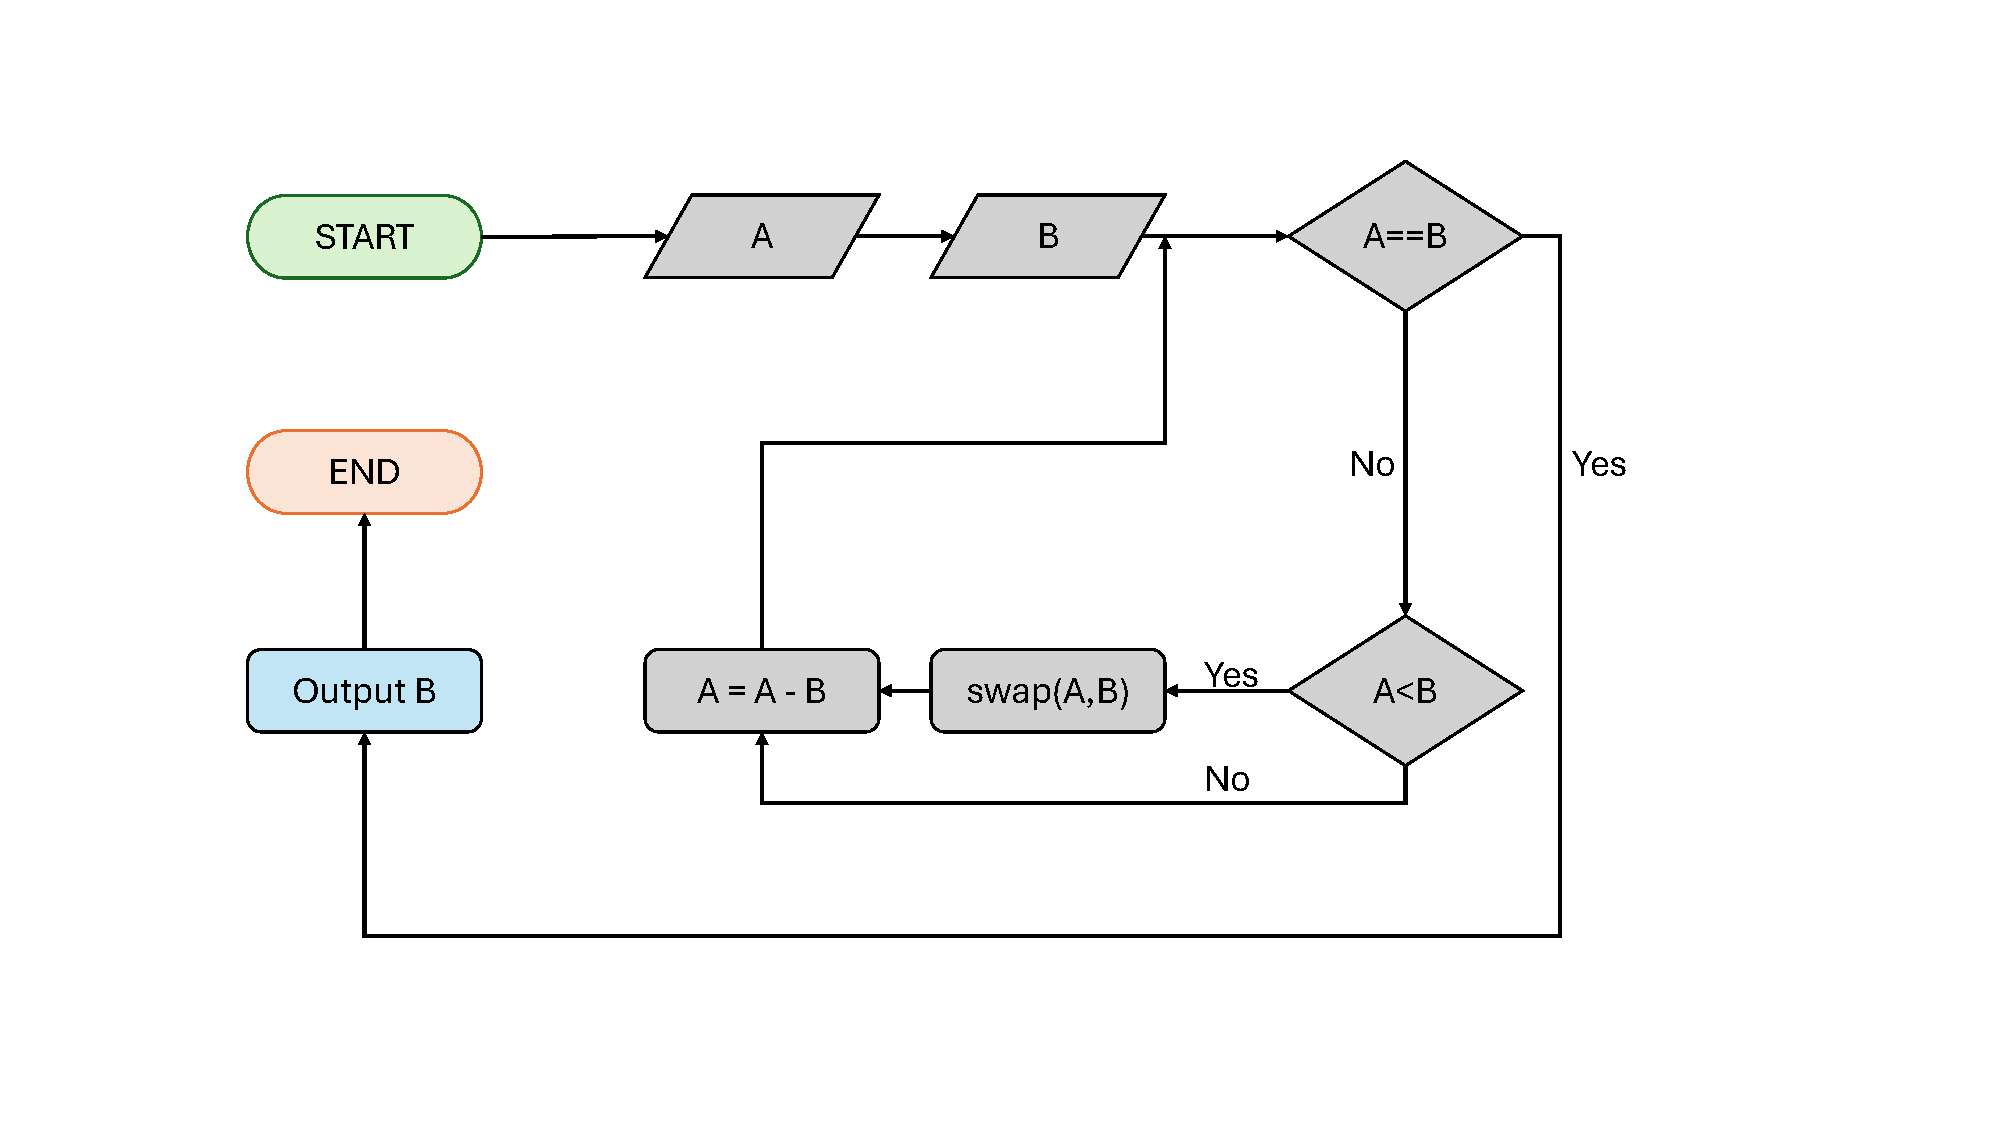
\includegraphics[width=.5\linewidth]{graphics/example.pdf}
  \caption{Example graphics.}
  \label{fig:example}
\end{figure}

Table stuff going in \Cref{tab:example} \lipsum[6]
\begin{table}
	\caption{Weird table title example.} 
	\label{tab:example}
	\begin{tabular}{lr}
		\toprule
		\multicolumn{2}{c}{Channel \hspace{2cm} Responses} \\ 
		\midrule
		DevOps Chat Slack & 3 \\ 
		Devops Weekly Newsletter & 24  \\ 
		Facebook & 3 \\ 
		LinkedIn & 7 \\ 
		\bottomrule
	\end{tabular}
\end{table}


\section{This is a section of a chapter}
\label{sec:intro:section}

\lipsum[7]

\subsection{This is a subsection of a section}
\label{sec:intro:subsection}

\lipsum[8]

\subsubsection{This is a sub-subsection of a subsection}
\label{sec:intro:subsubsection}

\lipsum[9]